\documentclass[12pt]{amsart}
\usepackage[T1]{fontenc}
\usepackage[utf8]{inputenc}

\usepackage[top=1.95cm, bottom=1.95cm, left=2.35cm, right=2.35cm]{geometry}

\usepackage{hyperref}
\usepackage{enumitem}
\usepackage{tcolorbox}
\usepackage{float}
\usepackage{cleveref}
\usepackage{multicol}
\usepackage{fancyvrb}
\usepackage{amsmath}
\usepackage[french]{babel}
\usepackage[
    type={CC},
    modifier={by-nc-sa},
	version={4.0},
]{doclicense}

\newcommand\floor[1]{\left\lfloor #1 \right\rfloor}

\usepackage{tnsmath}


\newtheorem{fact}{Fait}[section]
\newtheorem{example}{Exemple}[section]
\newtheorem{remark}{Remarque}[section]
\newtheorem*{proof*}{Preuve}

\setlength\parindent{0pt}

\floatstyle{boxed} 
\restylefloat{figure}


\DeclareMathOperator{\taille}{\text{\normalfont\texttt{taille}}}

\newcommand\sqseq[2]{\fbox{$#1$}_{\,\,#2}}


\DefineVerbatimEnvironment{rawcode}%
	{Verbatim}%
	{tabsize=4,%
	 frame=lines, framerule=0.3mm, framesep=2.5mm}
	 
	 
	 
\begin{document}

\title{BROUILLON - Sommer les carrés des chiffres d'un naturel}
\author{Christophe BAL}
\date{6 Juin 2018 -- 28 Mars 2019}

\maketitle

\begin{center}
	\itshape
	Document, avec son source \LaTeX, disponible sur la page
	
	\url{https://github.com/bc-writing/drafts}.
\end{center}


\bigskip


\begin{center}
	\hrule\vspace{.3em}
	{
		\fontsize{1.35em}{1em}\selectfont
		\textbf{Mentions \og légales \fg}
	}
			
	\vspace{0.45em}
	\doclicenseThis
	\hrule
\end{center}


\bigskip
\setcounter{tocdepth}{1}
\tableofcontents



\section{Faire une tête au carré à tous les entiers naturels}

Ci dessous, sur le cercle trigonométrique associé à un repère orthonormé $\paxes{O | I | J}$ , nous avons placé, les points $A$ , $B$ et $S$ de sorte que $\angleorient{\vect{OI}}{\vect{OS}} = \angleorient{\vect{OI}}{\vect{OA}} + \angleorient{\vect{OI}}{\vect{OB}}$ \emph{(cette construction est très naturelle)}.
Sauriez-vous conjecturer
\footnote{
	Le lieu de téléchargement de ce document contient un fichier GeoGebra \texttt{base-tool.ggb} manipulable dynamiquement pour vérifier combien il est aisé de conjecturer quelque chose.
}
un moyen simple de construire le point $S$ à partir des points $A$ et $B$ \emph{(la réponse est donnée dans la page suivante)} ?


\medskip

\begin{multicols}{2}
	\center

	\fbox{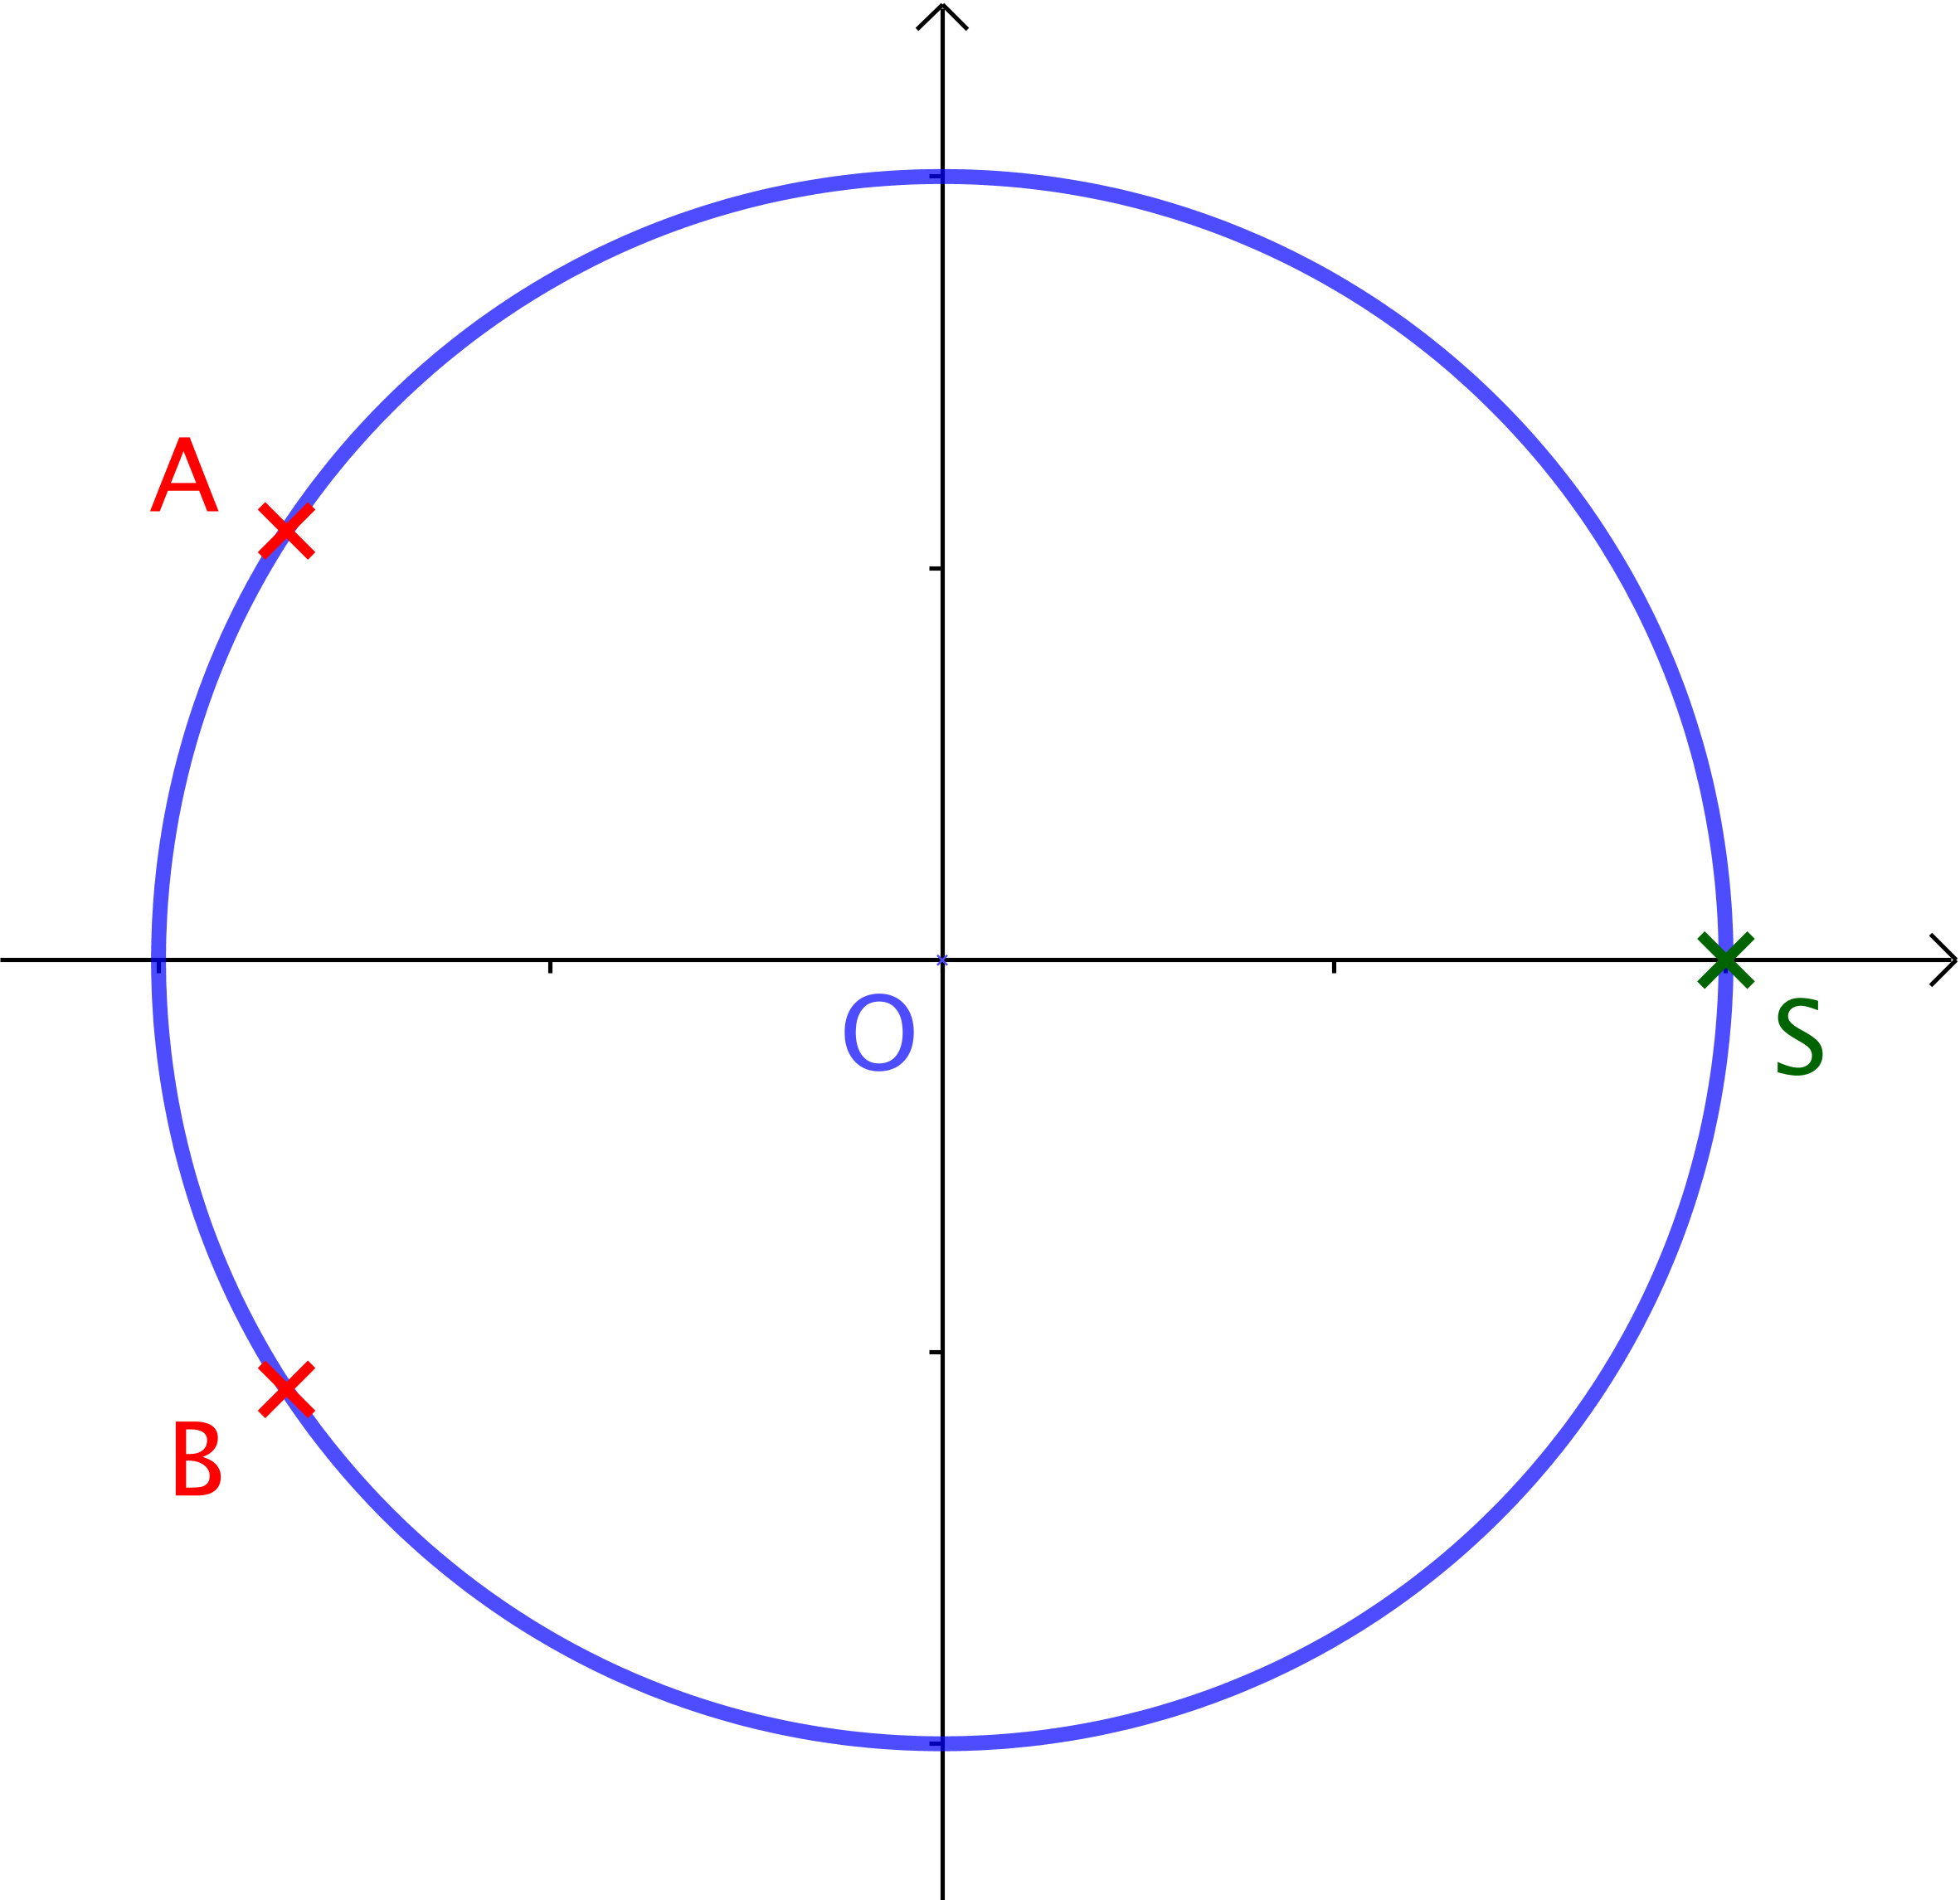
\includegraphics[scale = .75]{addition-on-ellipsis/conjecture/h-sym.png}}

	\columnbreak

	\fbox{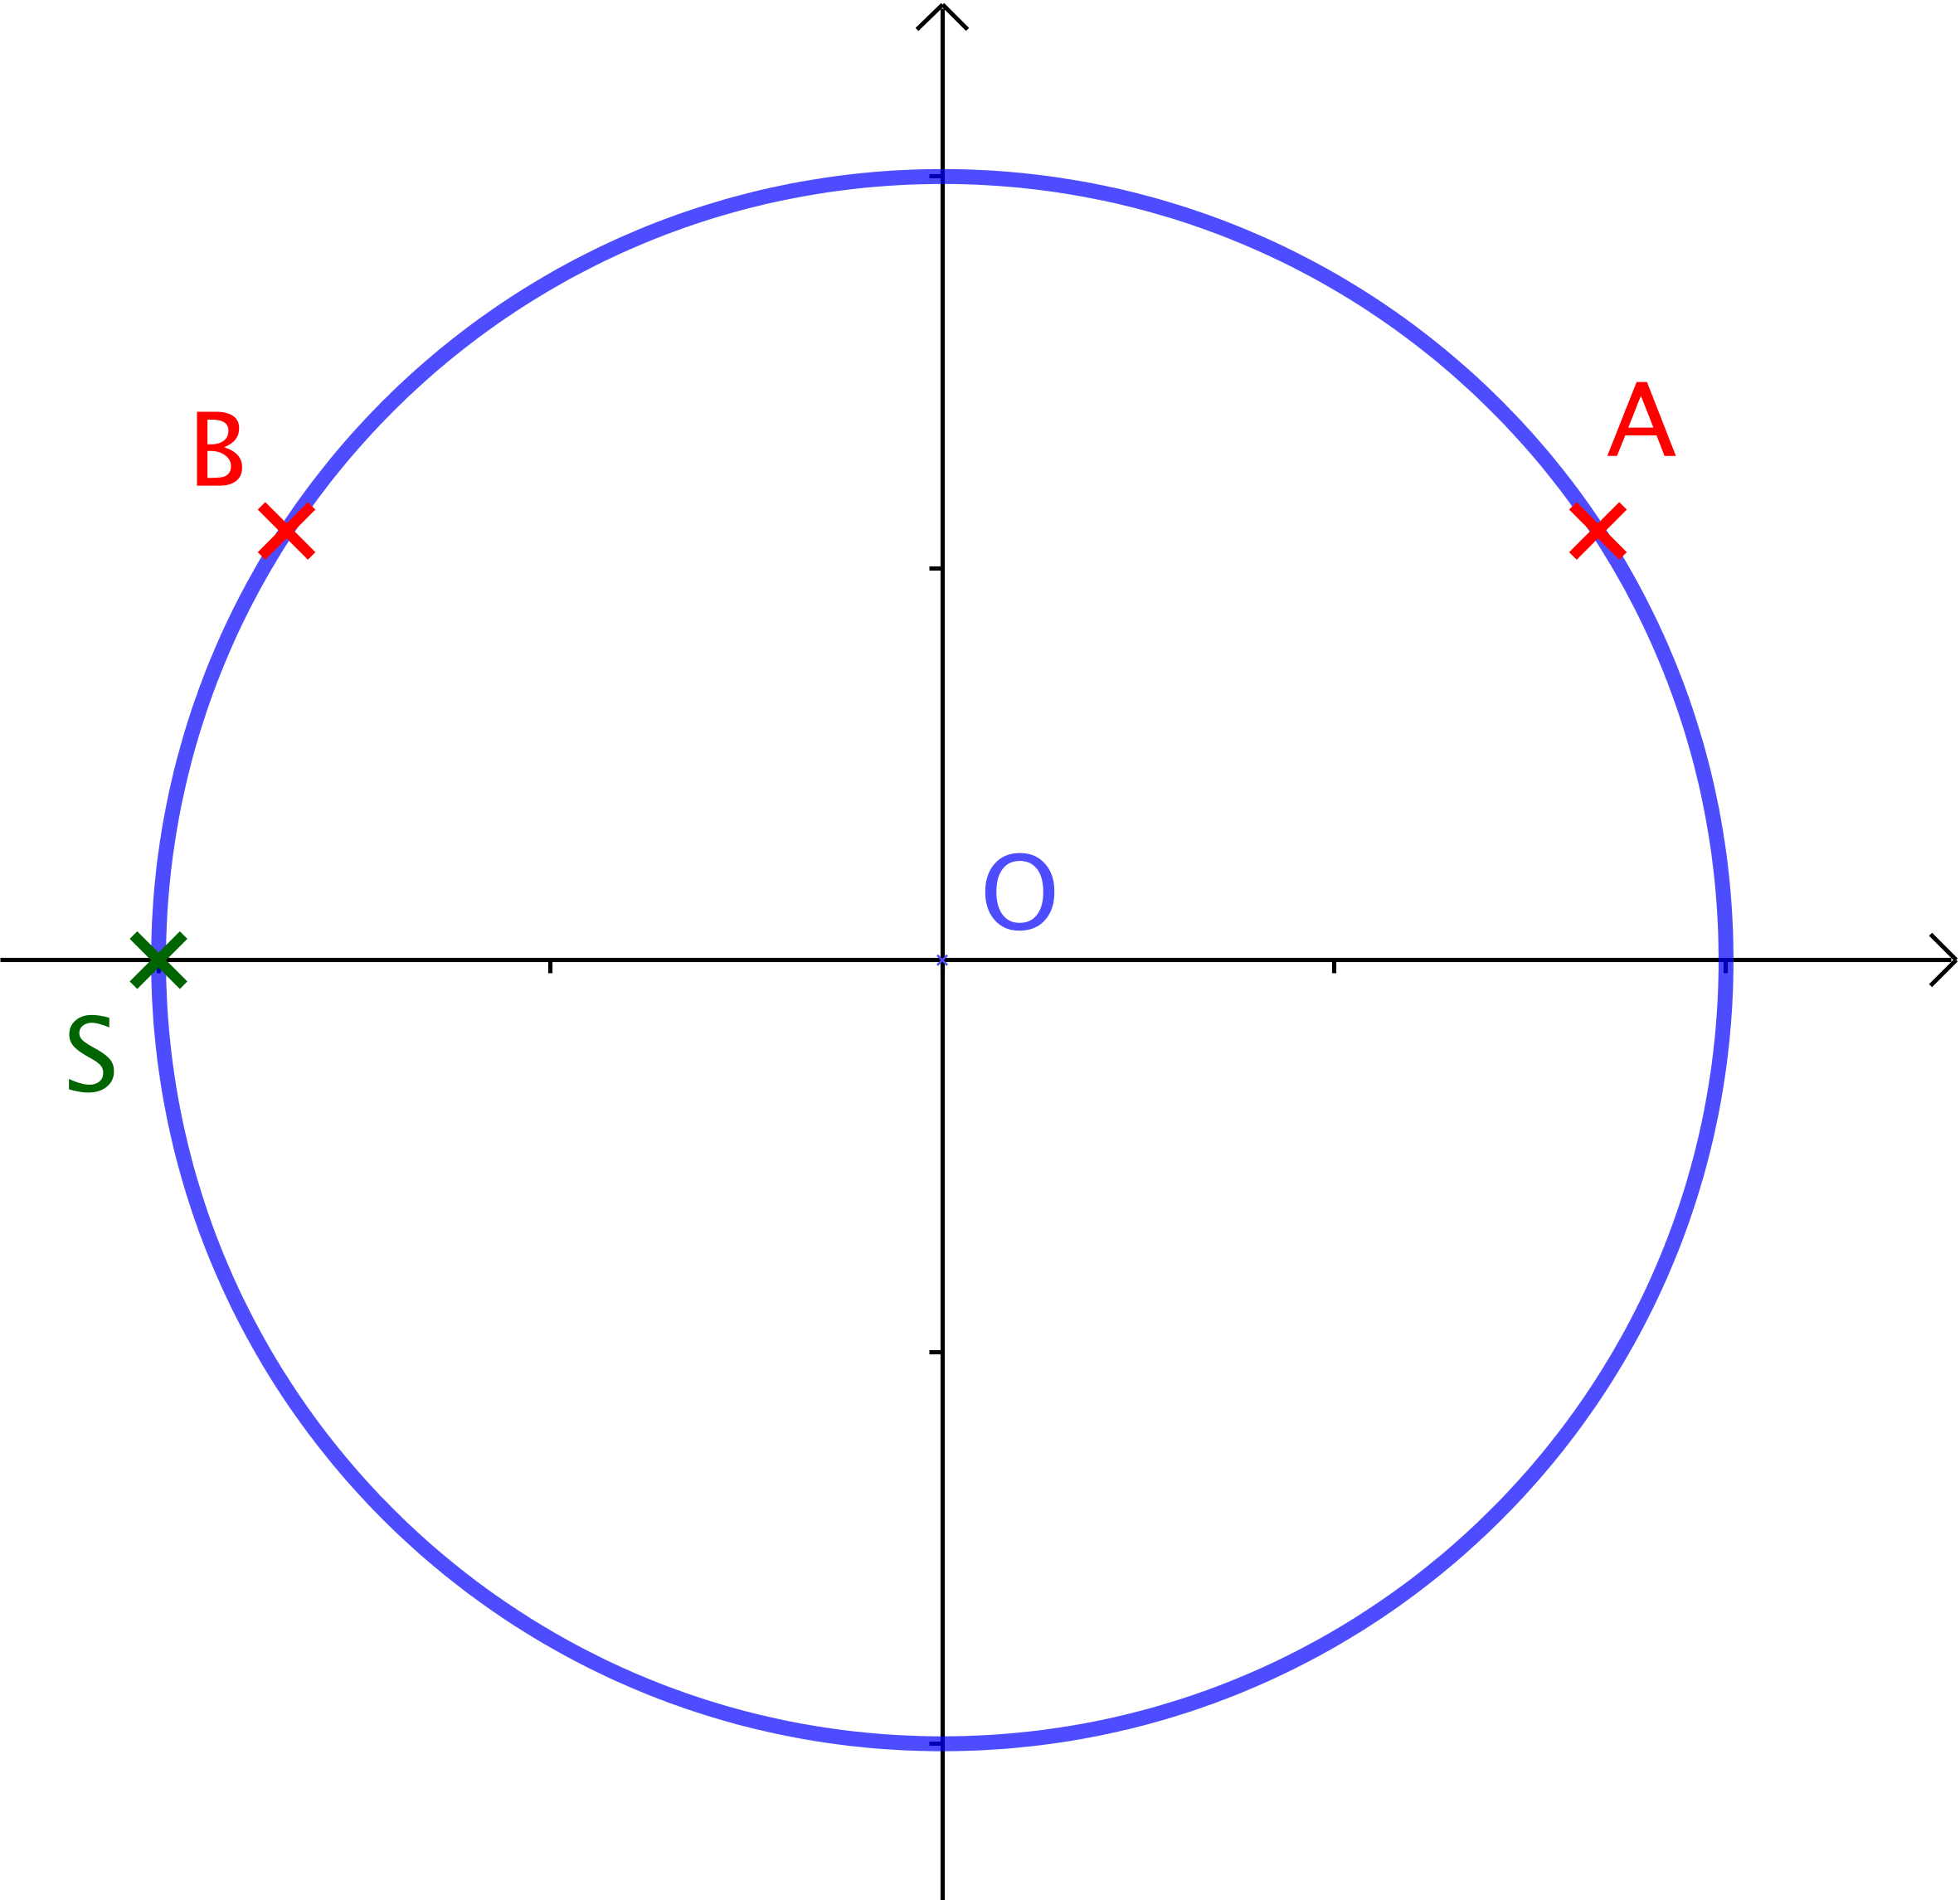
\includegraphics[scale = .75]{addition-on-ellipsis/conjecture/v-sym.png}}
\end{multicols}


\medskip

\begin{multicols}{2}
	\center

	\fbox{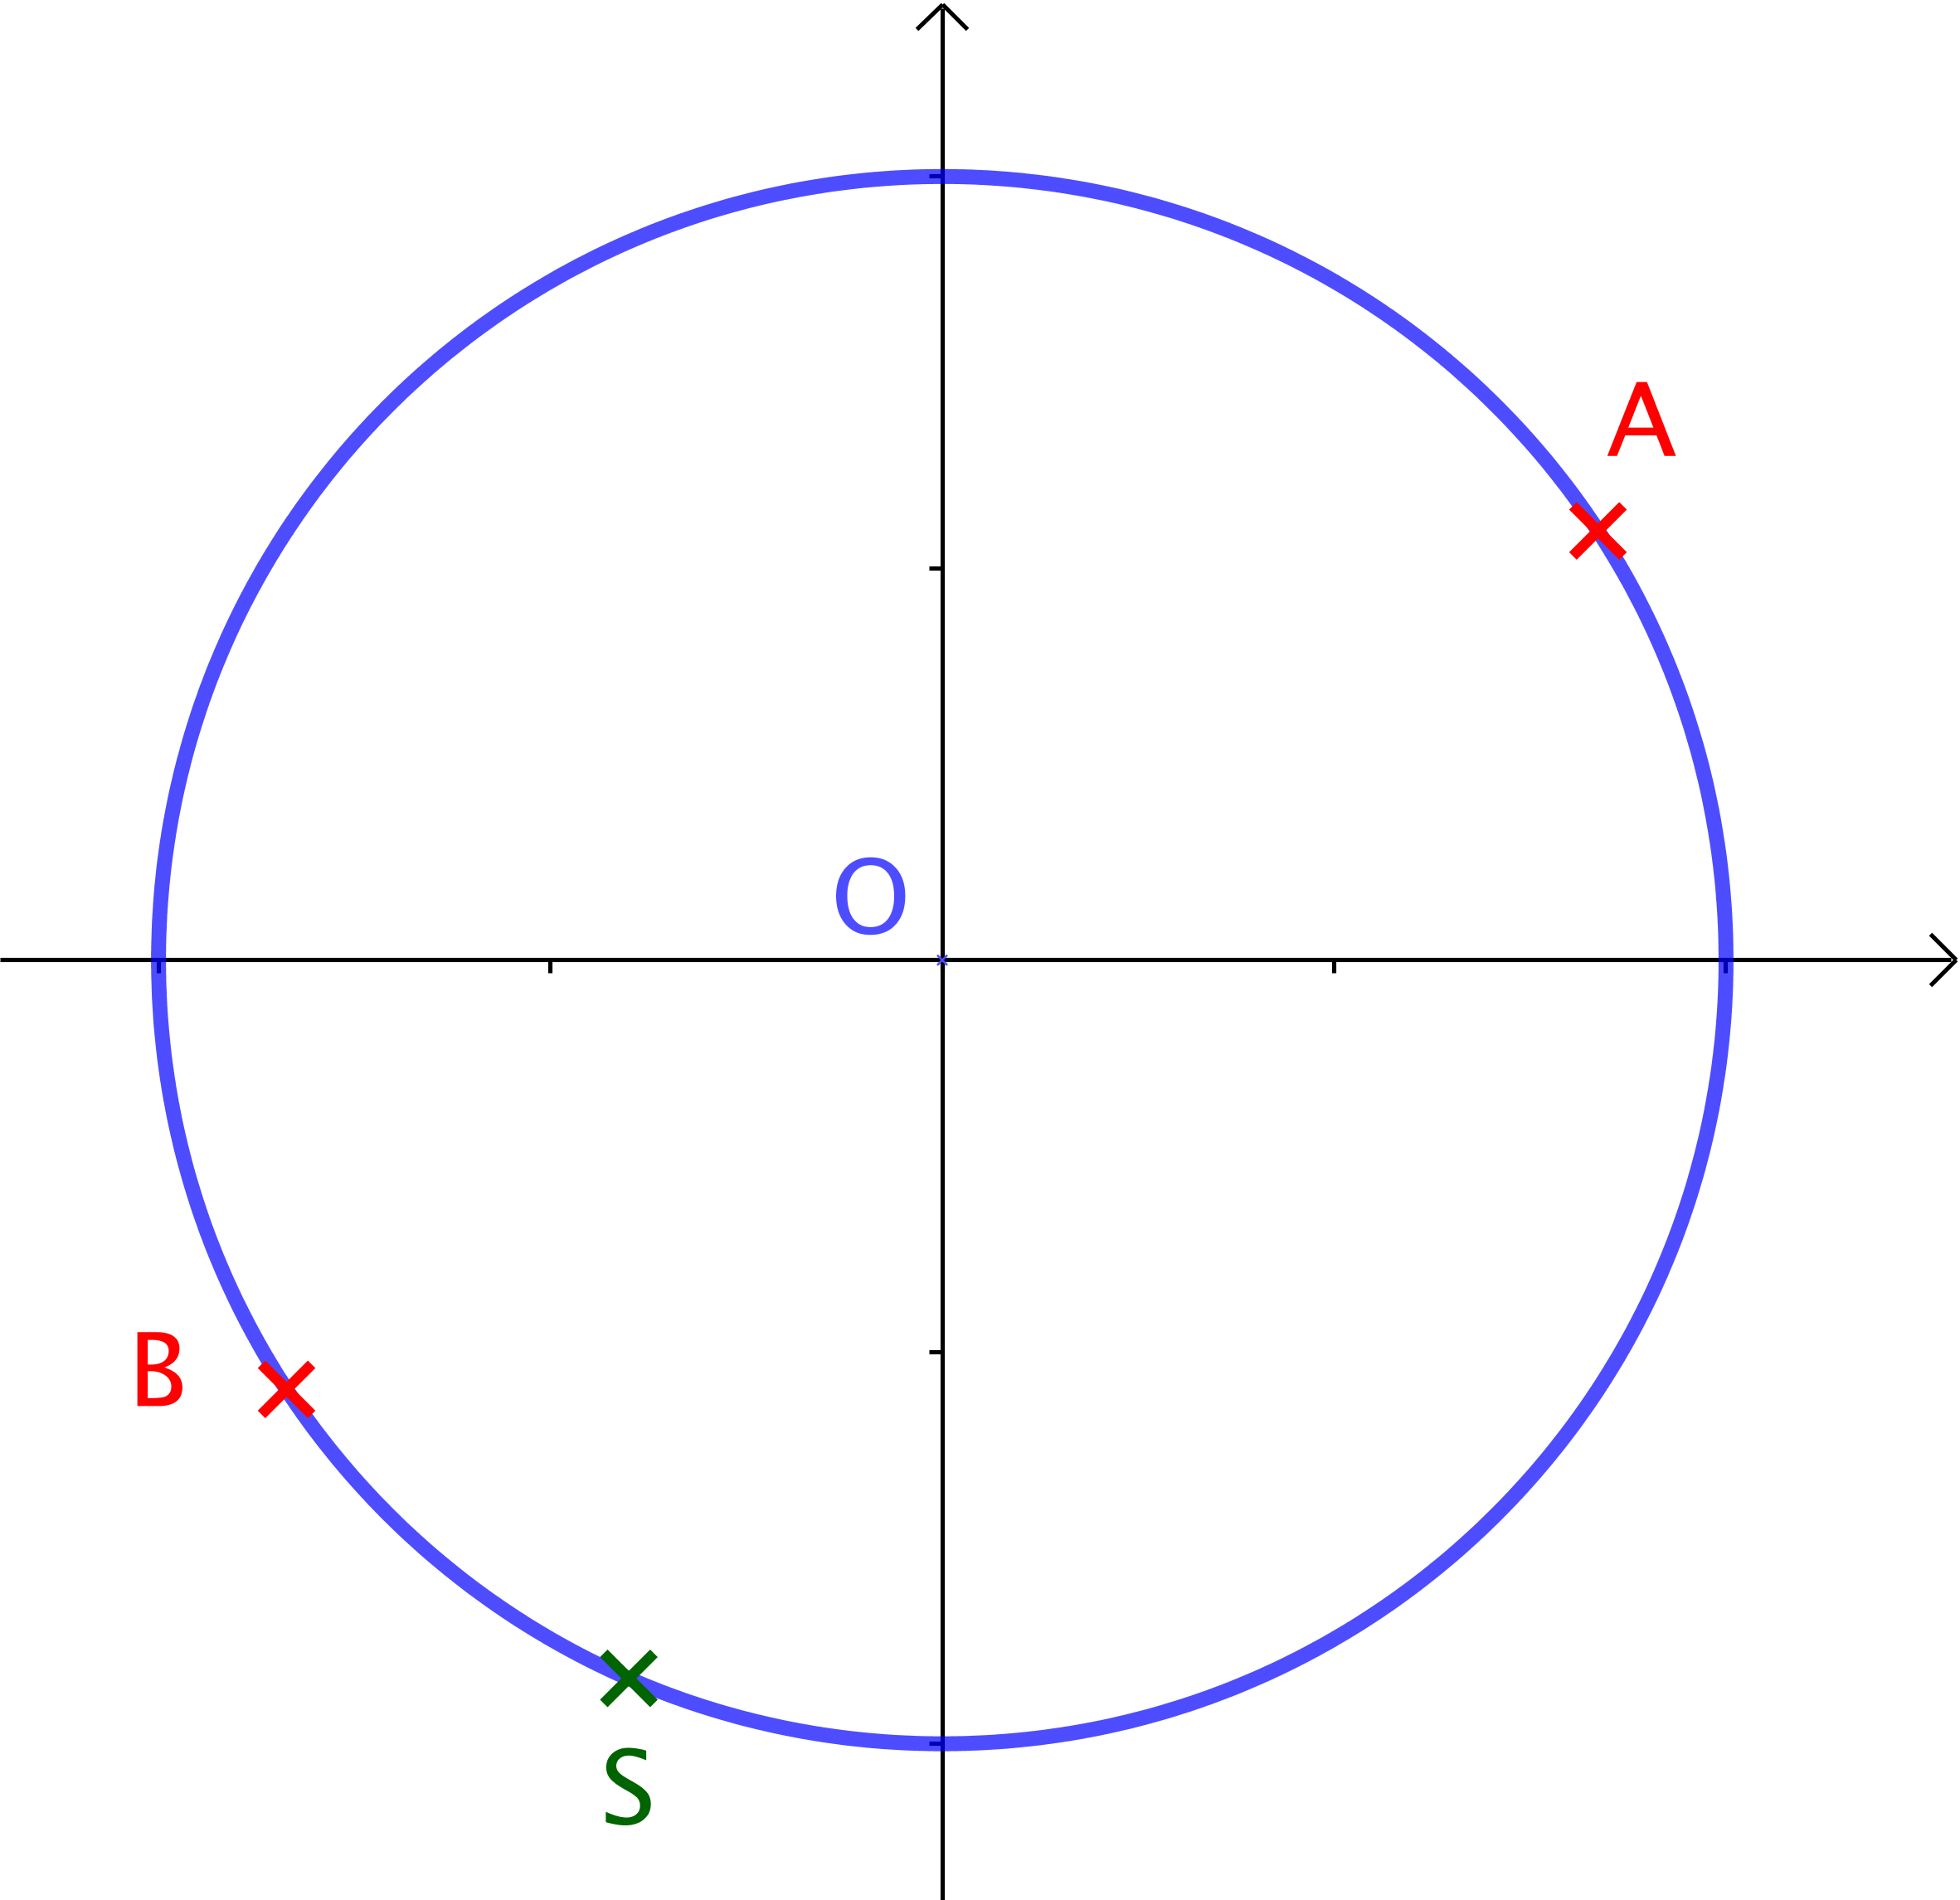
\includegraphics[scale = .75]{addition-on-ellipsis/conjecture/O-sym.png}}

	\columnbreak

	\fbox{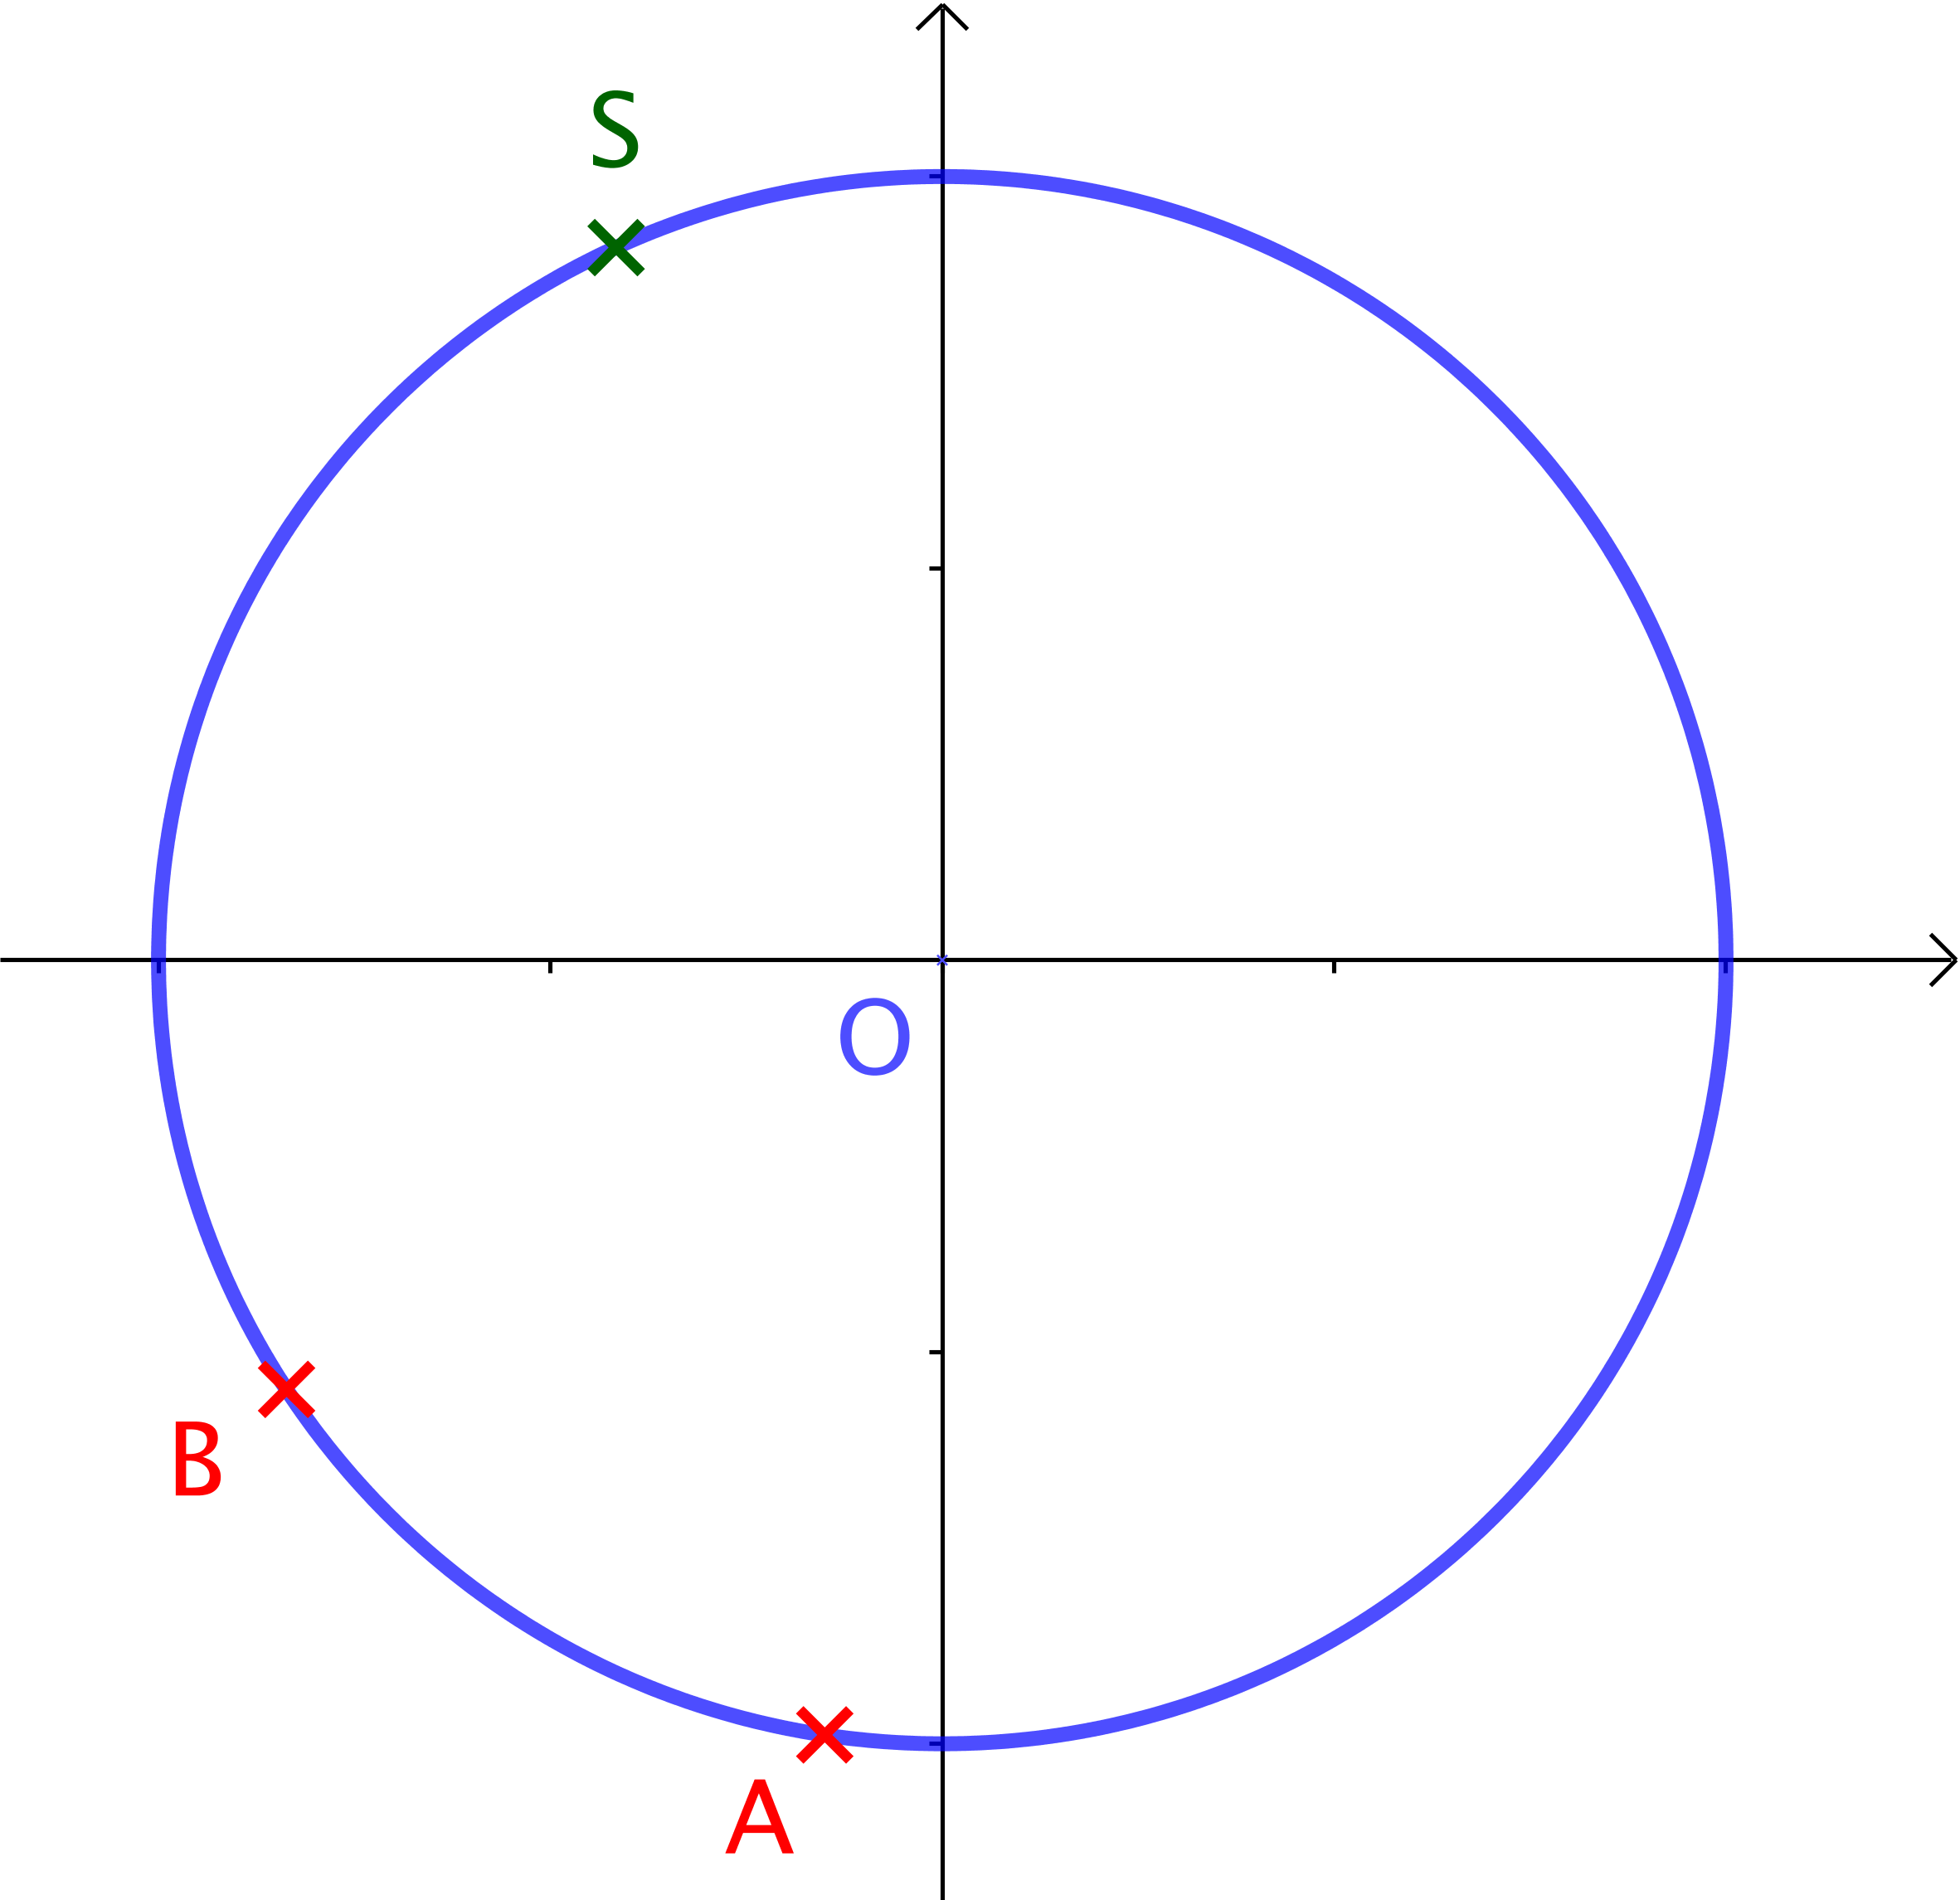
\includegraphics[scale = .75]{addition-on-ellipsis/conjecture/general.png}}
\end{multicols}


\newpage

Pour mieux voir ce qu'il se passe, il suffit de tracer quelques droites. Voici ce que cela donne.

\begin{multicols}{2}
	\center

	\fbox{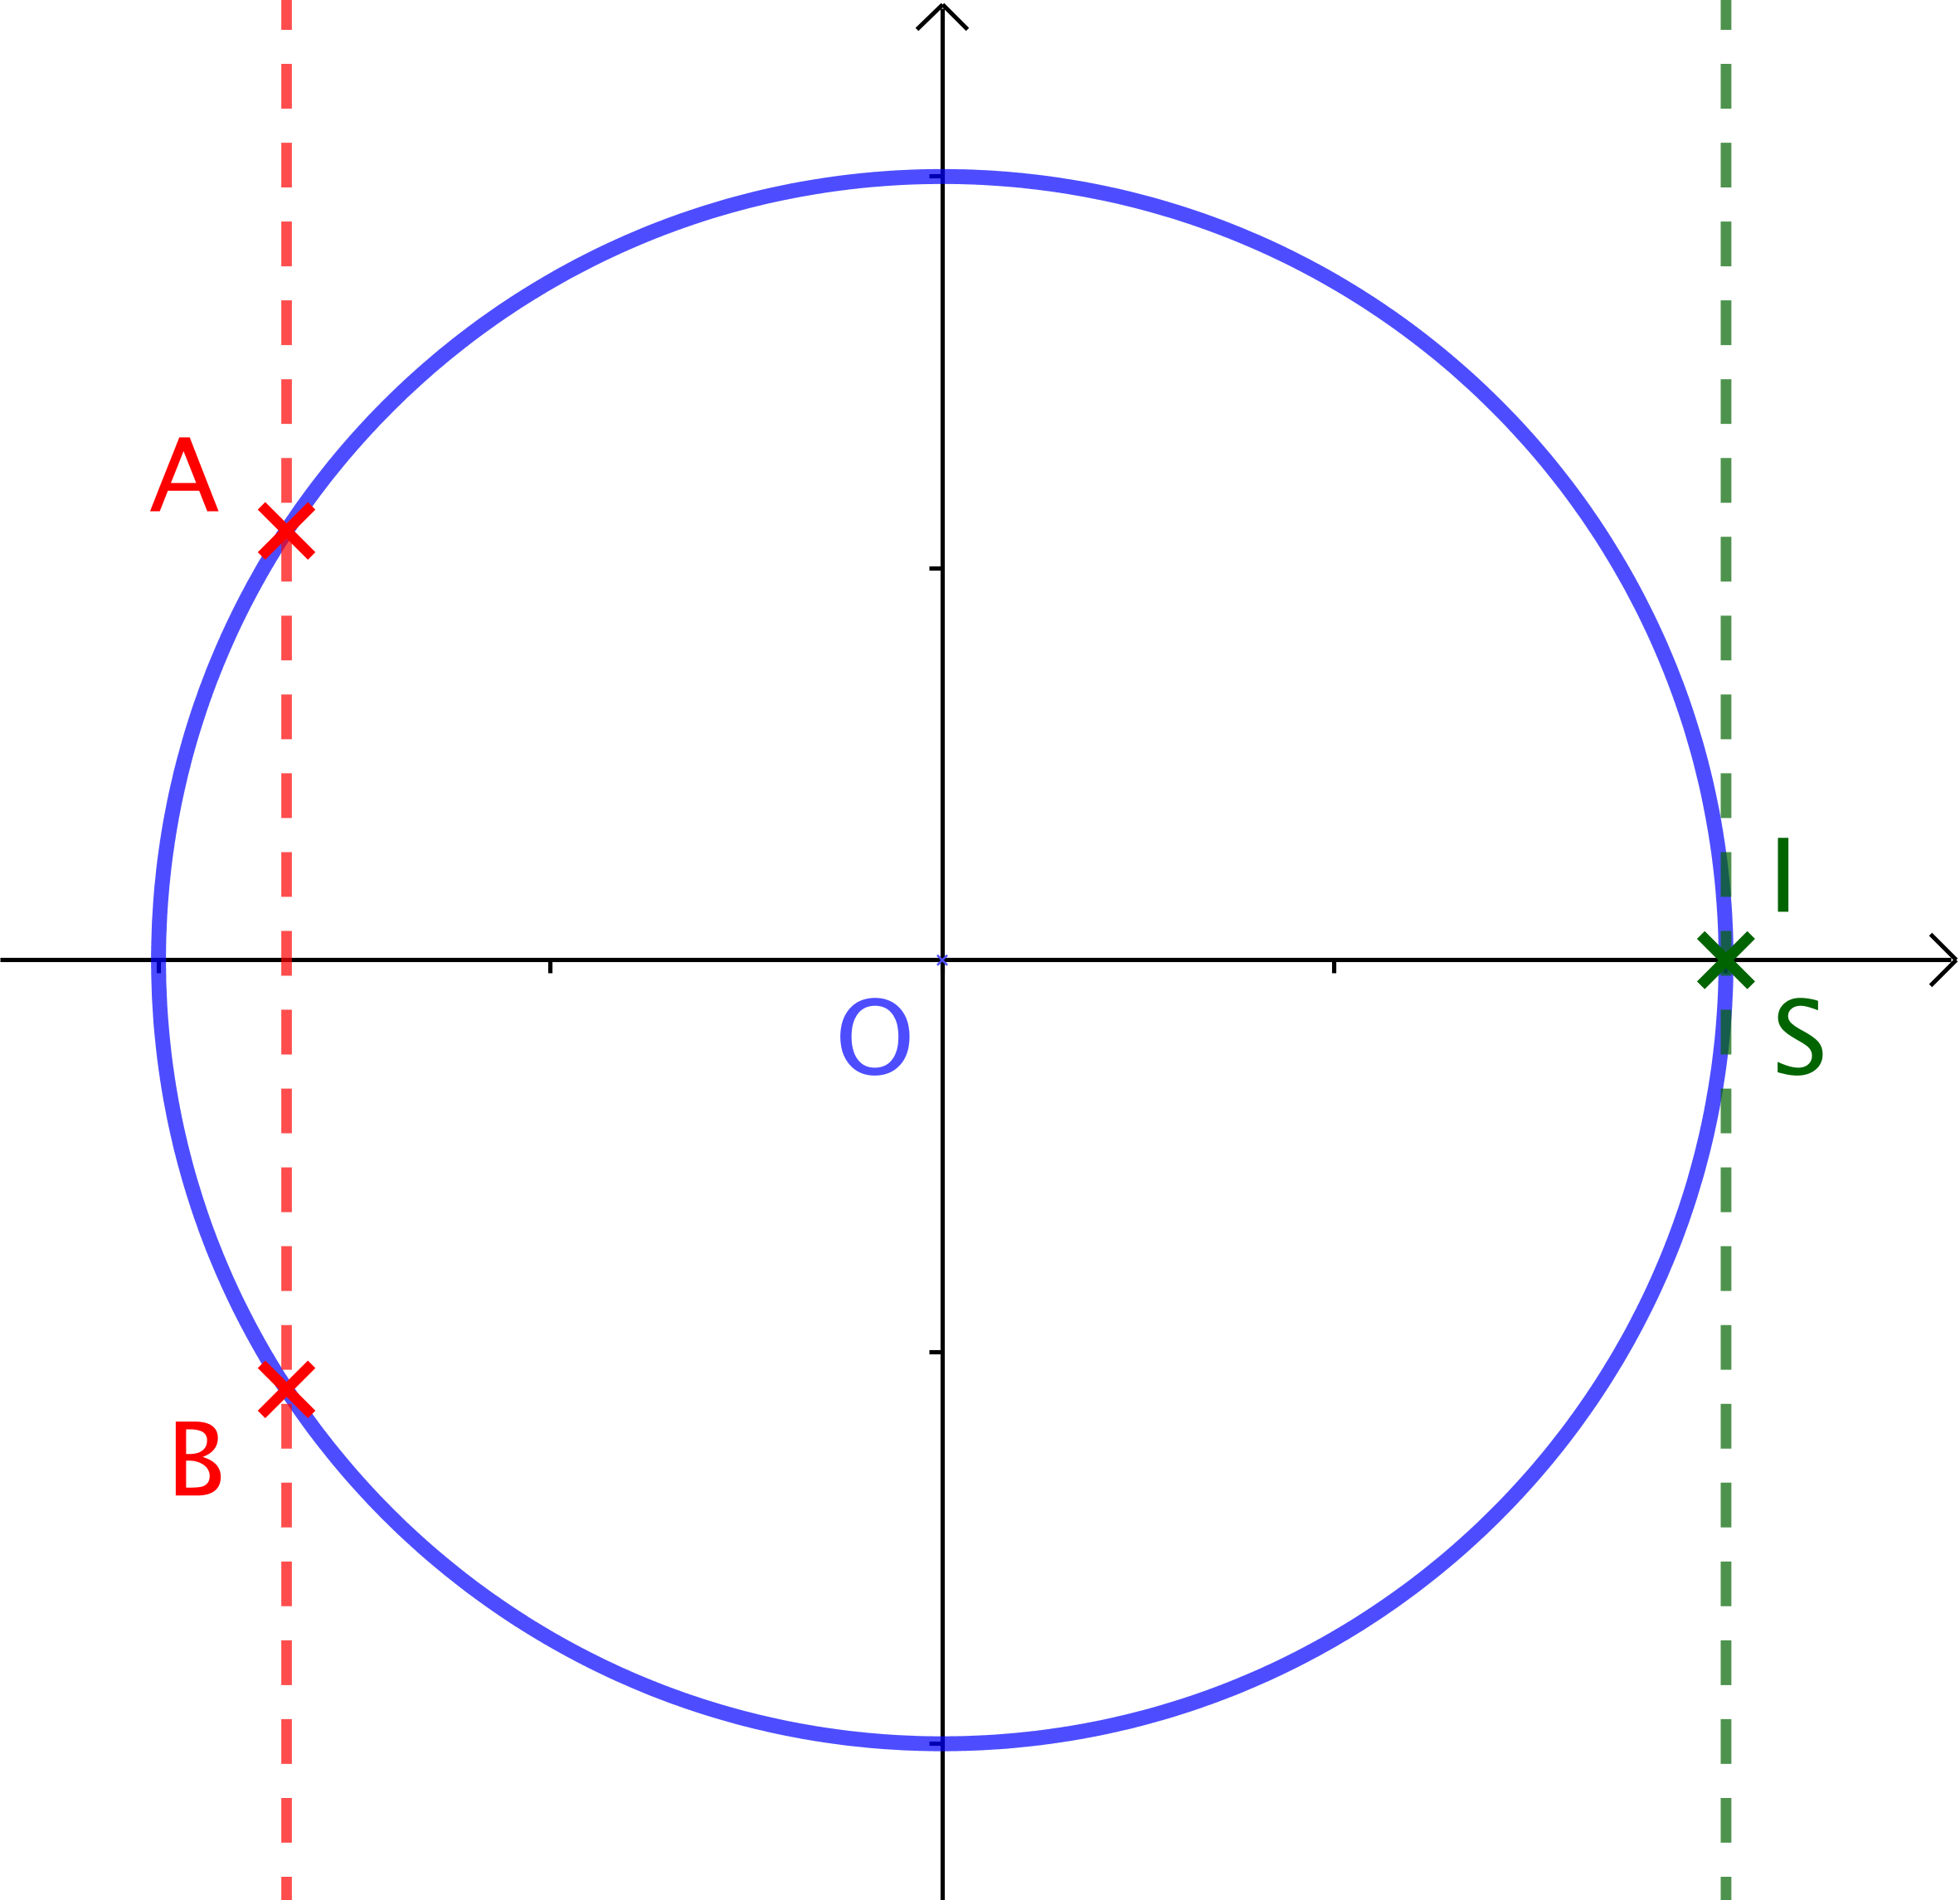
\includegraphics[scale = .75]{addition-on-ellipsis/conjecture/h-sym-with-lines.png}}

	\columnbreak

	\fbox{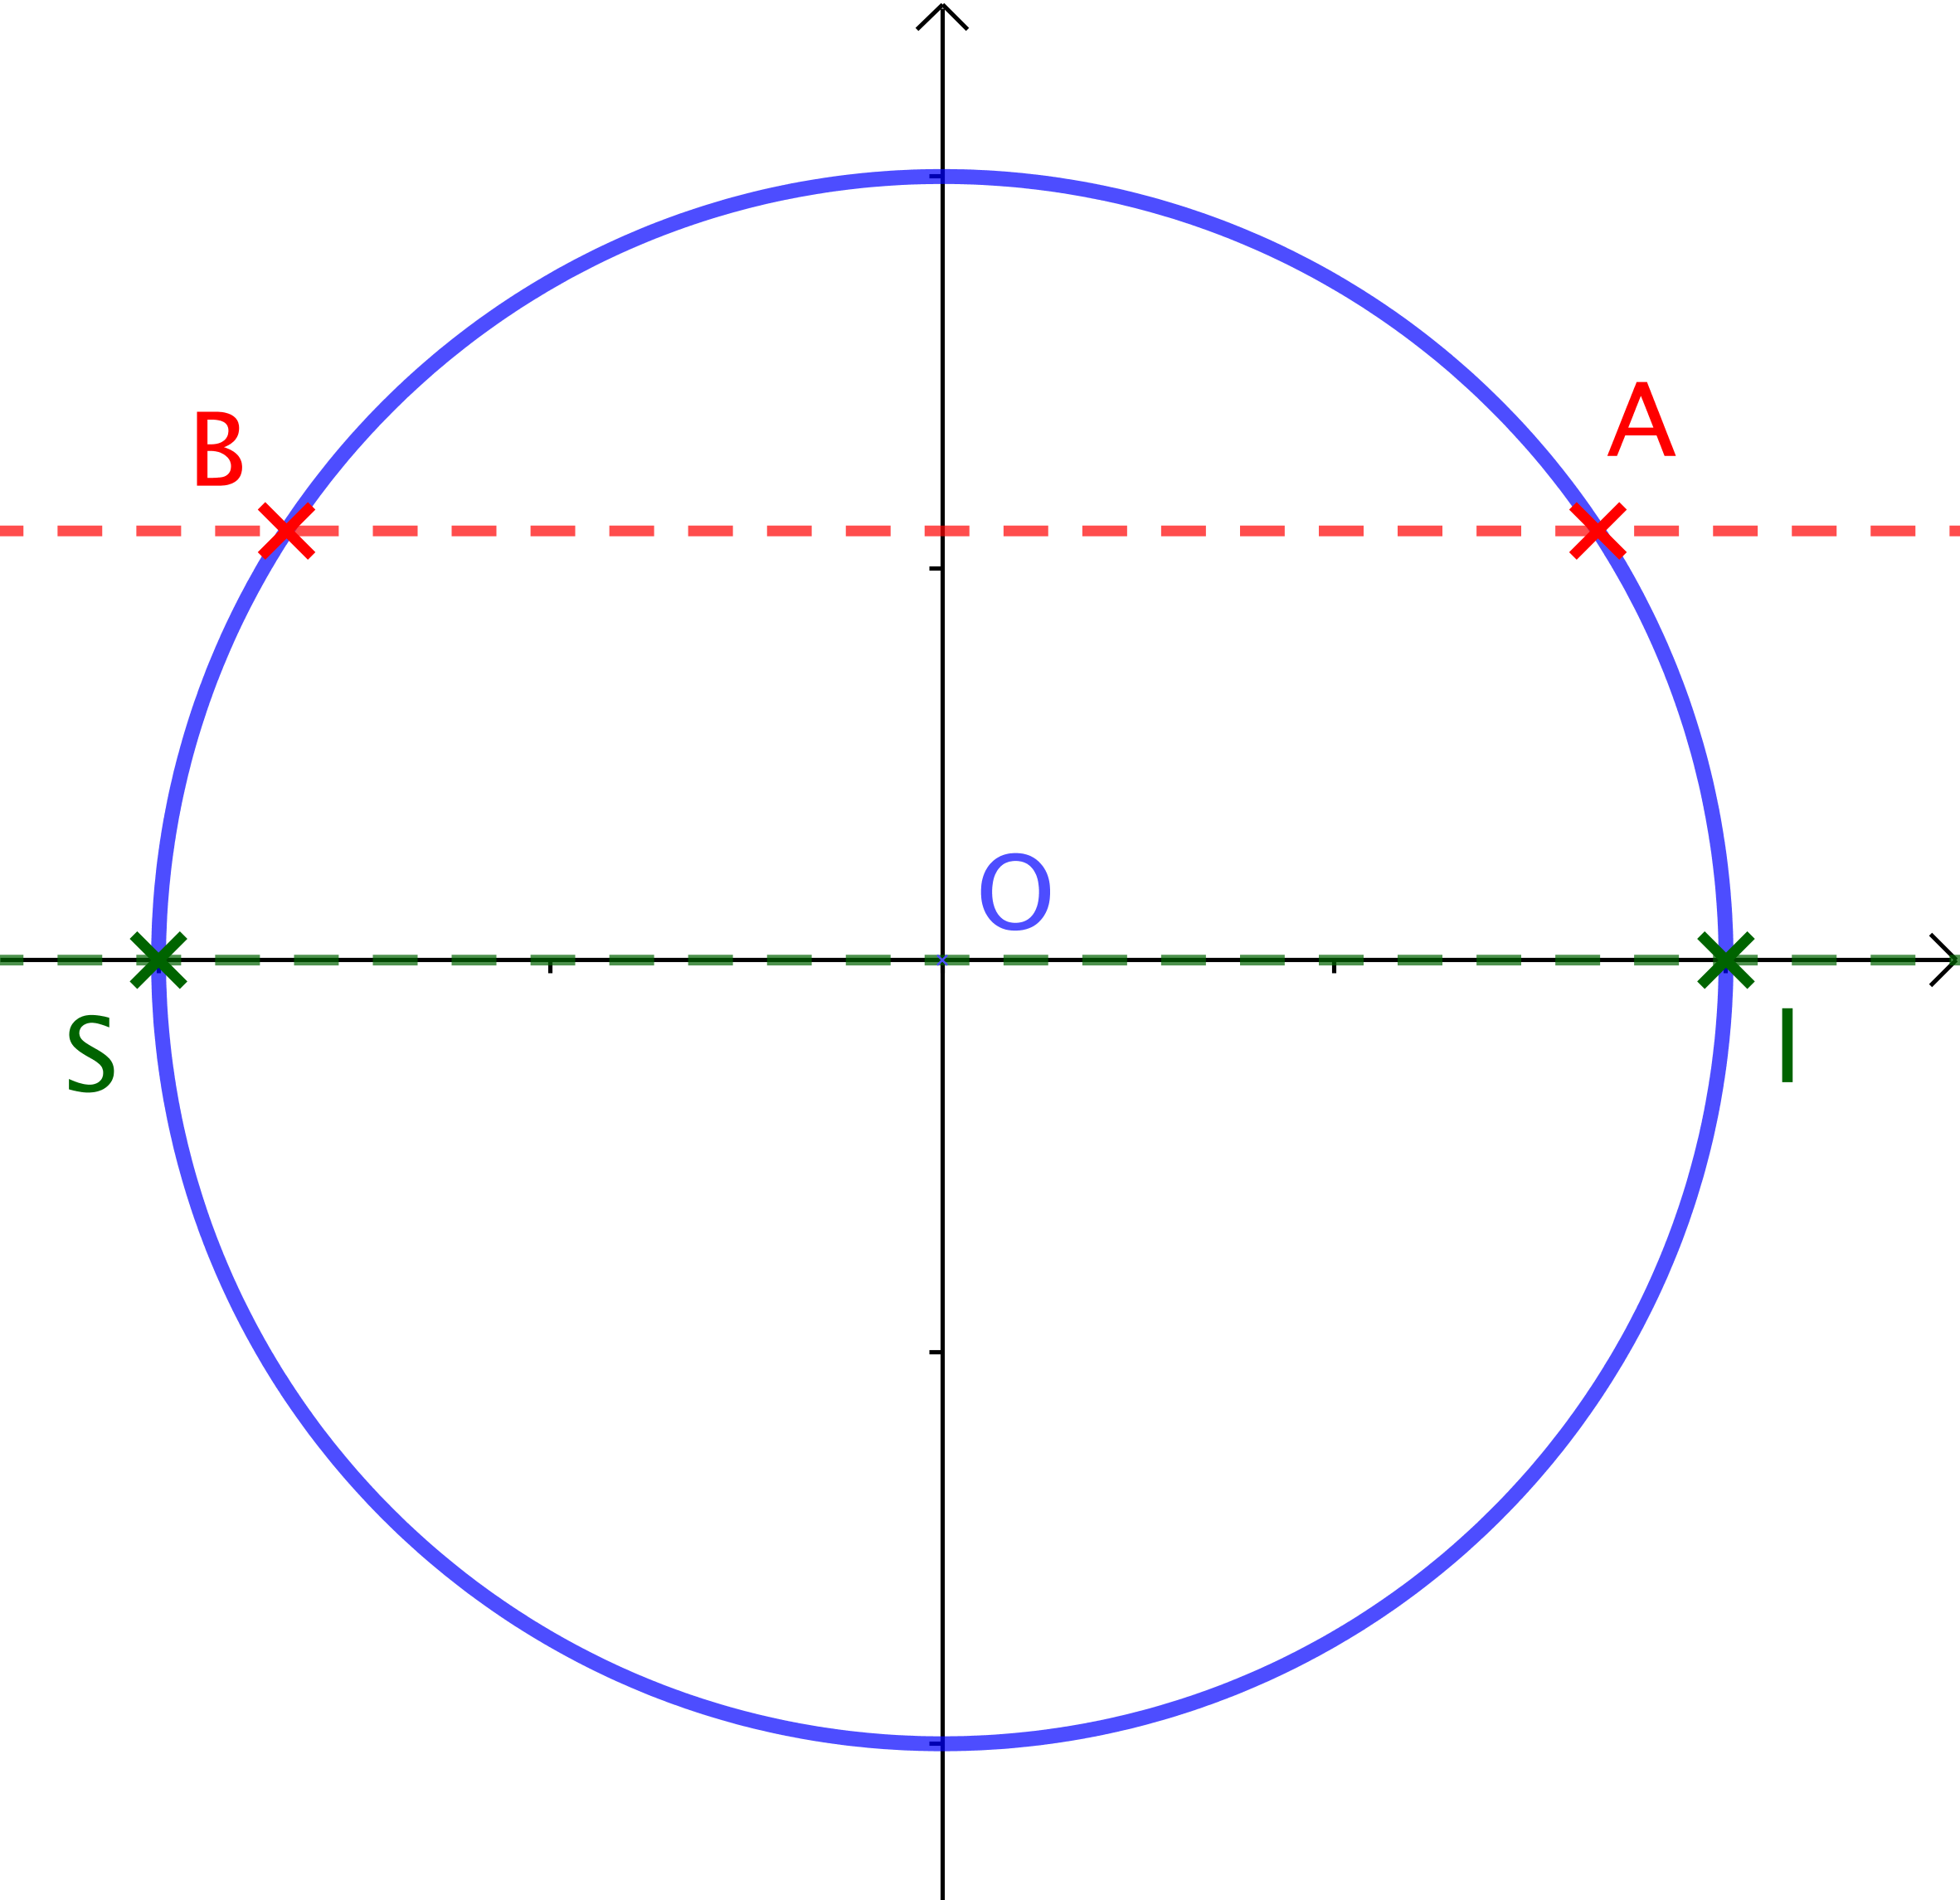
\includegraphics[scale = .75]{addition-on-ellipsis/conjecture/v-sym-with-lines.png}}
\end{multicols}


\medskip

\begin{multicols}{2}
	\center

	\fbox{\includegraphics[scale = .75]{addition-on-ellipsis/conjecture/o-sym-with-lines.png}}

	\columnbreak

	\fbox{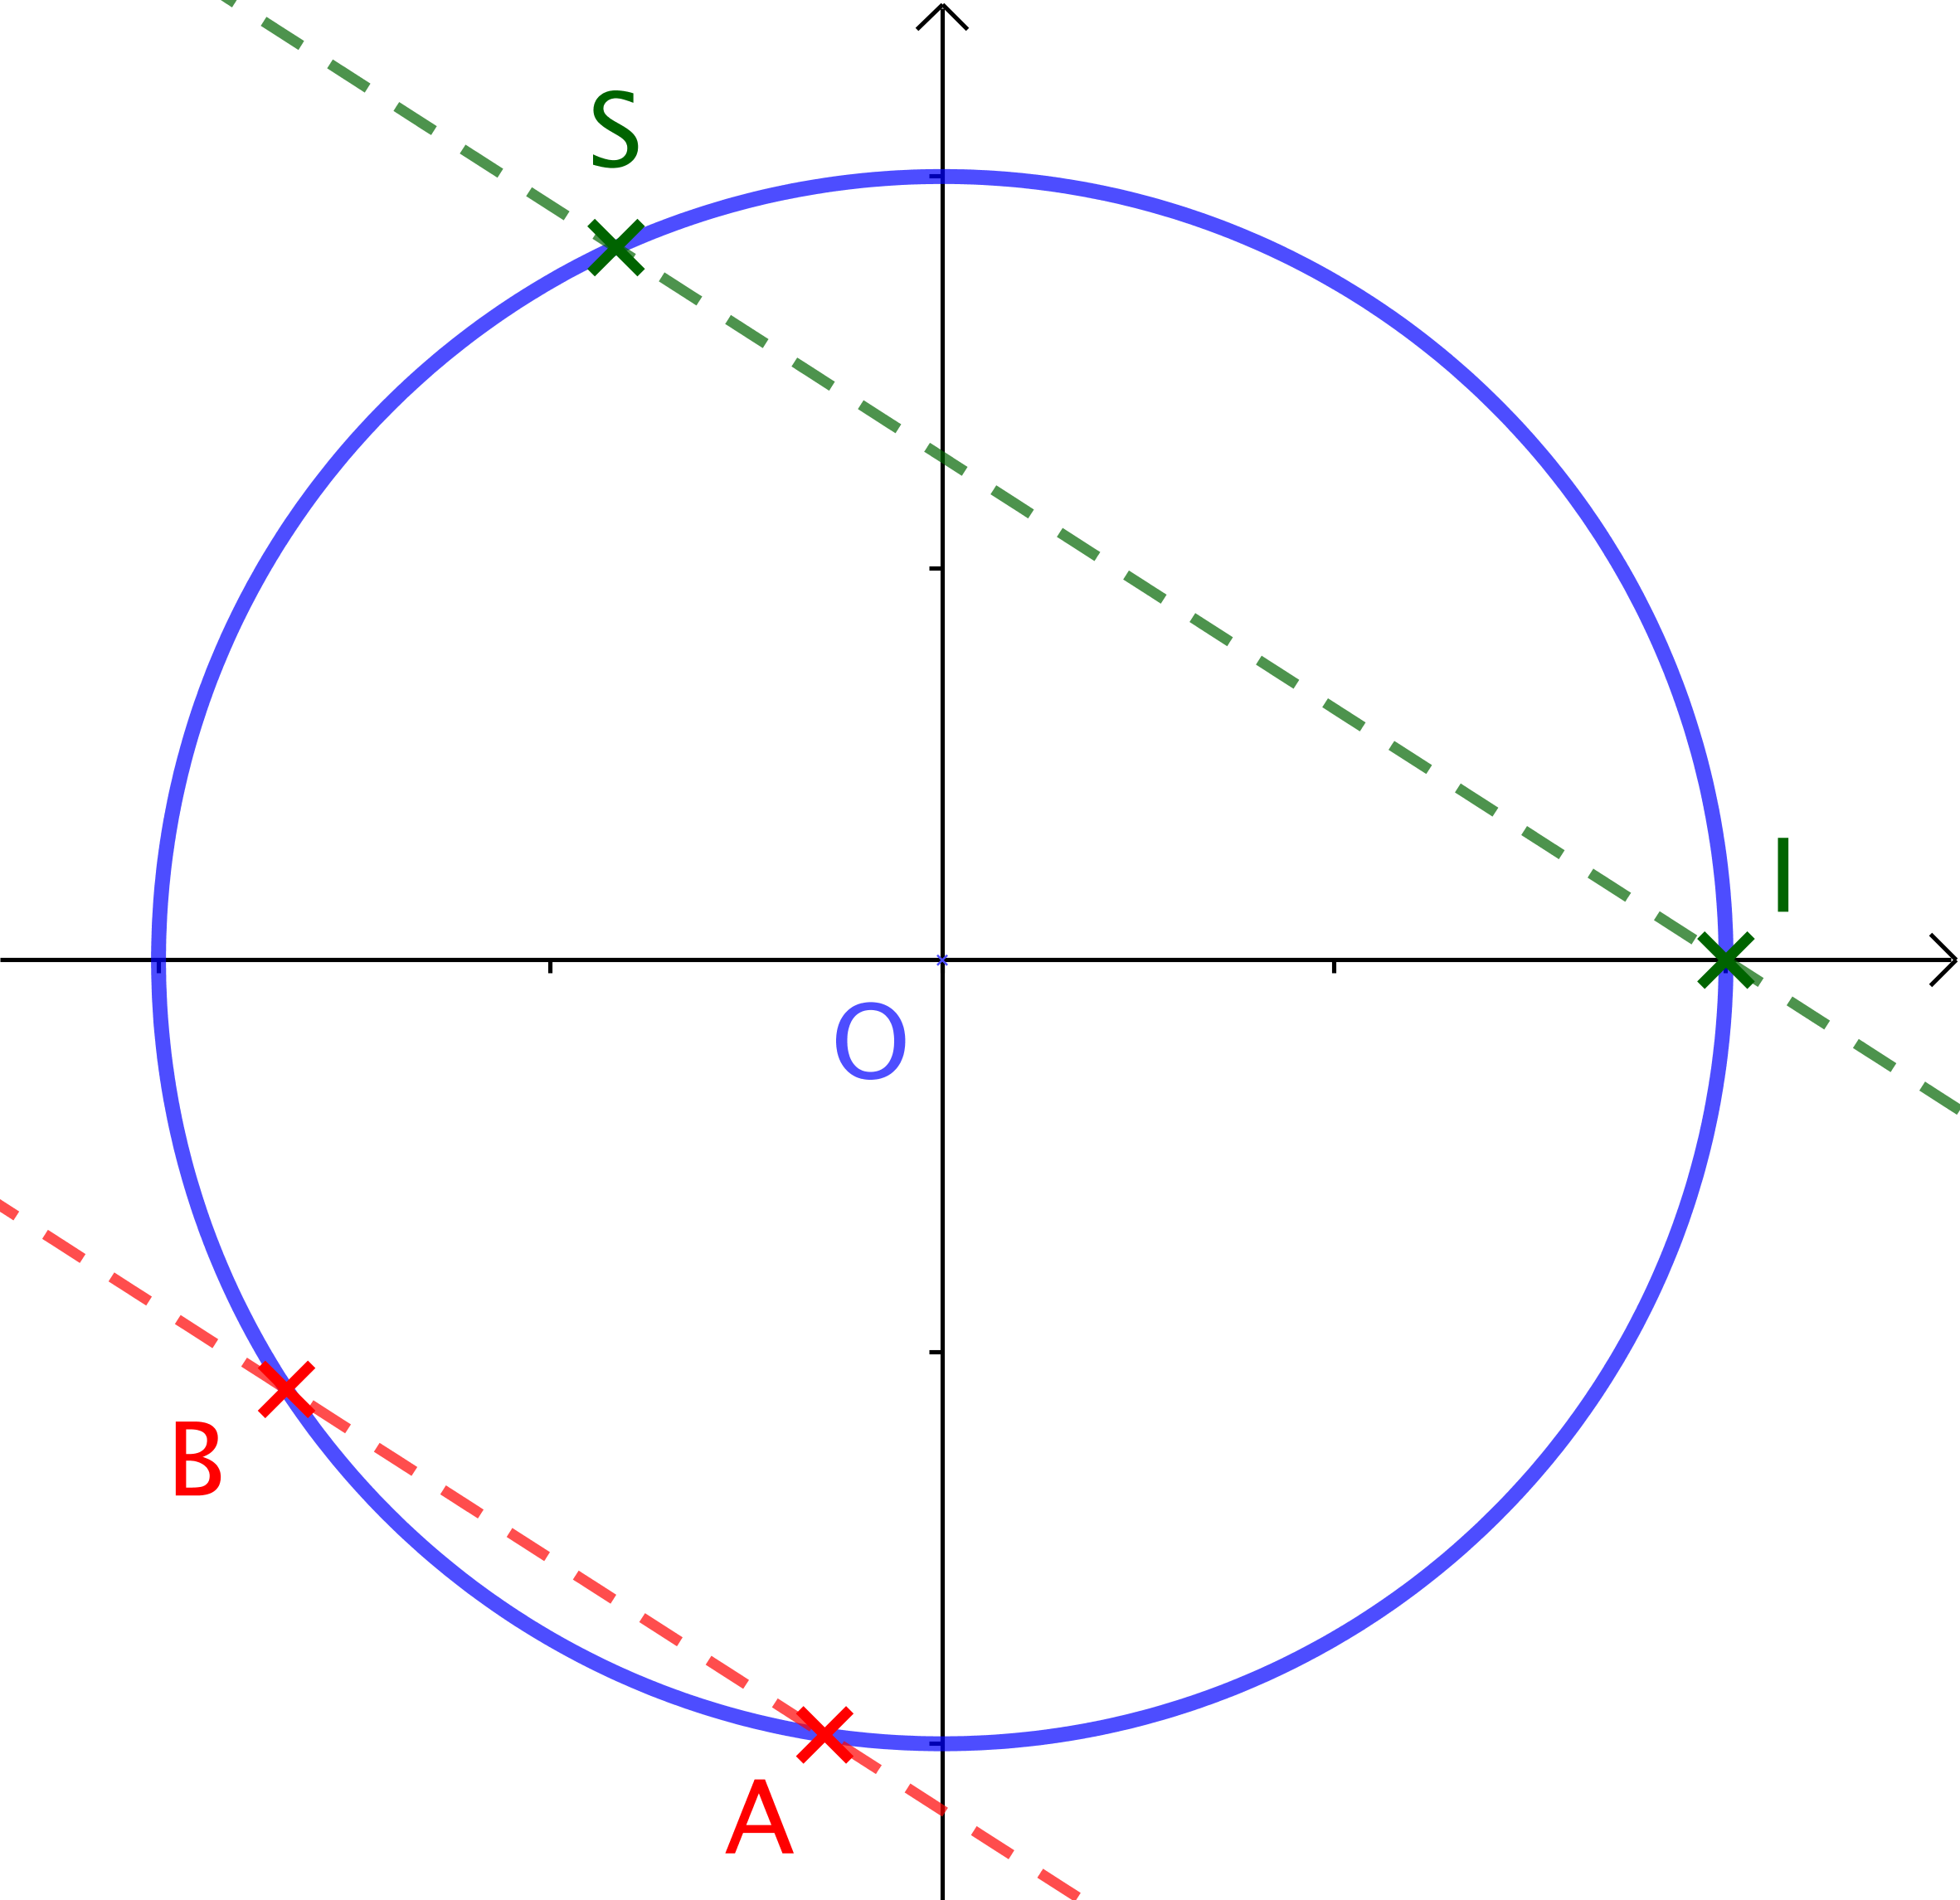
\includegraphics[scale = .75]{addition-on-ellipsis/conjecture/general-with-lines.png}}
\end{multicols}


Il devient évident de conjecturer que le point $S$ se construit géométriquement comme suit.

\begin{enumerate}
	\item \label{point-1} Si $A \neq B$ alors on construit la parallèle à $(AB)$ passant par $I$ . 
	Si cette parallèle n'est pas tangente au cercle alors le point $S$ est le second point d'intersection de cette parallèle avec le cercle, sinon $S = I$ .
	Notons que dans le second cas, c'est à dire si $x_A = x_B$ et $y_A = -y_B$ , alors $S = I$ peut être vu comme un point d'intersection \squote{double}.

	\item Si $A = B$ , on procède comme au point (\ref{point-1}) mais avec la parallèle à la tangente en $A$ au cercle. Intuitivement, cette situation consiste à faire \emph{\og tendre \fg} $A$ vers $B$ 
	\footnote{
		Nous évitons les arguments faisant appel à l'analyse afin de rester dans un cadre géométrique le plus général possible.
	}.
\end{enumerate}


\medskip

Dans ce qui suit nous allons valider cette conjecture de trois façons en allant du plus brutal au plus élégant.

\begin{enumerate}
	\item La 1\iere{} méthode passe assez brutalement via les critères de colinéarité et d'orthogonalité dans un plan.
	
	\item La 2\ieme{} méthode utilise les nombres complexes avec des calculs faciles à mener.
	
	\item La 3\ieme{} méthode, sûrement la plus élégante, est purement géométrique.
\end{enumerate}
\label{conjecture}


\section{Une preuve}\label{proof}

Rappelons que $\setgeo{H} : y = \frac{1}{x}$ , $E(1 ; 1)$ , $A \left( a ; \frac{1}{a} \right)$ , $B \left( b ; \frac{1}{b} \right)$ et $P \left( p ; \frac{1}{p} \right)$ où $p = a b$ avec $(a ; b) \in \left( \RRs \right)^2$ .



\bigskip

\textbf{Cas 1.} \emph{Supposons que $x_A x_B = 1$ .}

\medskip

Il est clair que $P = E$ dans ce cas.



\bigskip

\textbf{Cas 2.} \emph{Supposons que $x_A x_B \neq 1$ et $A \neq B$ .}

\medskip

La droite $(AB)$ a pour pente
$\frac{y_A - y_B}{x_A - x_B} = \frac{1}{a - b} \left( \frac{1}{a} - \frac{1}{b} \right) = - \frac{1}{ab}$ .
De plus, la droite $(EP)$ , qui existe car $p \neq 1$ , a pour pente
$\frac{y_P - y_E}{x_P - x_E} = \frac{1}{p - 1} \left( \frac{1}{p} - 1 \right) = - \frac{1}{p} = - \frac{1}{ab}$ .
Les droites $(AB)$ et $(EP)$ sont bien parallèles comme nous l'avons affirmé.



\bigskip

\textbf{Cas 3.} \emph{Supposons que $x_A x_B \neq 1$ et $A = B$ .}

\medskip

Comme ici $p = a^2 \neq 1$ . la droite $(EP)$ a pour pente $\left( - \frac{1}{a^2} \right)$ qui est aussi la pente de la tangente en $A \left( a ; \frac{1}{a} \right)$ à l'hyperbole $\setgeo{H}$ comme annoncé. 


\section{Coder - Étudier la \og période \fg{} d'un naturel}

\input{squares-digits/period}


\section{\texorpdfstring{Peut-on généraliser à un exposant $k \geqslant 3$ ?}%
		                {Peut-on généraliser à un exposant k >= 3 ?}}

\input{squares-digits/bigger-power}




\bigskip

\hrule

\section{AFFAIRE À SUIVRE...}

\bigskip

\hrule


%\section{Quelles périodes déterminées informatiquement}
%
%\input{squares-digits/bigger-power-some-periods}

\end{document}
